\subsectiuneclasa{Clasa a XI-a}{Șiruri, limite, continuitate, derivabilitate.}{Enunțuri · Clasa a XI-a}
\nivelE{olm}{Nivelul OLM}
\prob{olm}{OLM.1}{Clasică}
\begin{parti}
  \item Fie $f:\mathbb{R}\to\mathbb{R}$ o funcție continuă cu proprietatea că $f(x+q)=f(x)$ pentru orice $x\in\mathbb{R}$ și orice $q\in\mathbb{Q}$. Demonstrați că $f$ este constantă.
  \item Există funcții $f:\mathbb{R}\to\mathbb{R}$ neconstante, periodice cu perioade oricât de mici (adică pentru orice $\varepsilon>0$ există $0<p<\varepsilon$ cu $f(x+p)=f(x)$ pentru orice $x$)? Dacă în plus $f$ este continuă, mai este posibil?
\end{parti}
\vspace{1mm}\hrule

\prob{olm}{OLM.2}{Clasică}
Fie șirul $x_1=\sqrt{2}$, $x_{n+1}=\sqrt{2+x_n}$.
\begin{parti}
  \item Arătați că șirul este convergent și calculați limita sa.
  \item Calculați $\displaystyle\lim_{n\to\infty}4^{\,n}\bigl(2-x_n\bigr)$.
\end{parti}
\vspace{1mm}\hrule

\prob{olm}{OLM.3}{}
Fie $(x_n)_{n\ge0}$ un șir de numere reale cu $x_{n+2}=x_{n+1}-x_n$ pentru orice $n\ge0$. Arătați că șirul este periodic și exprimați $x_{2026}$ în funcție de $x_0$ și $x_1$.
\vspace{1mm}\hrule

\prob{olm}{OLM.4}{}
Fie $n\ge1$ un număr natural. Arătați că ecuația
\[ x^{2n+1}+x^{2n-1}+x=1 \]
are exact o soluție reală și că aceasta se află în intervalul $(0,1)$.
\vspace{1mm}\hrule

\prob{olm}{OLM.5}{Clasică}
Arătați că nu există nicio funcție derivabilă $f:\mathbb{R}\to\mathbb{R}$ cu $f'(x)=\operatorname{sgn}(x)$ pentru orice $x\in\mathbb{R}$ (unde $\operatorname{sgn}$ ia valorile $-1$, $0$, respectiv $1$, după cum argumentul este negativ, nul sau pozitiv).
\vspace{1mm}\hrule

\prob{olm}{OLM.6}{}
Arătați că ecuația
\[ e^x=1+x+\frac{x^2}{2}+\frac{x^3}{6} \]
are exact o soluție reală.
\vspace{1mm}\hrule

\prob{olm}{OLM.7}{}
Arătați că ecuația
\[ x^{4}-4x+1=0 \]
are exact două soluții reale și că, notându-le $\alpha<\beta$, are loc $\alpha<1<\beta$.
\vspace{1mm}\hrule

\prob{olm}{OLM.8}{}
Fie $f:\mathbb{R}\to\mathbb{R}$ derivabilă, neidentic nulă, cu
\[ \lim_{x\to-\infty}f(x)=\lim_{x\to+\infty}f(x)=0 . \]
Arătați că există $c\in\mathbb{R}$ cu $f'(c)=0$.
\vspace{1mm}\hrule

\prob{olm}{OLM.9}{Clasică}
Fie $a_n=\dfrac{(n!)^{2}}{(2n)!}$, $n\ge1$.
\begin{parti}
  \item Calculați $\displaystyle\lim_{n\to\infty}a_n$ și $\displaystyle\lim_{n\to\infty}\binom{2n}{n}^{\!1/n}$.
  \item Arătați că $\sqrt{3n+1}\ \le\ 4^{\,n}a_n\ \le\ 2\sqrt n$ pentru orice $n\ge1$.
  \item Deduceți că $\displaystyle\lim_{n\to\infty}\frac{1}{4^{\,n}}\binom{2n}{n}=0$, dar $\displaystyle\lim_{n\to\infty}\frac{n}{4^{\,n}}\binom{2n}{n}=\infty$.
\end{parti}
\vspace{1mm}\hrule

\prob{olm}{OLM.10}{}
\begin{parti}
  \item Calculați $\displaystyle\lim_{x\to\infty}\ x\left(\frac{\pi}{2}-\arctan x\right)$.
  \item Arătați că $\displaystyle\lim_{n\to\infty}\ n\left(\frac{\pi}{2}-\arctan n\right)=1$, justificând trecerea de la limita de funcție la limita de șir.
  \item Redemonstrați limita de la (b) direct, folosind Cesàro--Stolz în cazul $\dfrac00$.
\end{parti}
\vspace{1mm}\hrule

\prob{olm}{OLM.11}{}
Fie $x_{1}\ge0$ și
\[ x_{n+1}=1+\frac{1}{1+x_{n}}\ ,\qquad n\ge1 . \]
\begin{parti}
  \item Arătați că șirul este convergent și calculați limita sa.
  \item Arătați că $\bigl|x_{n}-\sqrt2\bigr|\ \le\ 4^{\,2-n}$ pentru orice $n\ge2$.
\end{parti}
\vspace{1mm}\hrule

\prob{olm}{OLM.12}{Clasică}
Calculați $\displaystyle\lim_{n\to\infty}\sum_{k=1}^{n}\sin\frac{k}{n^2}$.
\vspace{1mm}\hrule

\prob{olm}{OLM.13}{}
Fie $f:\mathbb{R}\to\mathbb{R}$ o funcție continuă și periodică (există $T>0$ cu $f(x+T)=f(x)$ pentru orice $x$), pentru care limita $\displaystyle\lim_{x\to+\infty}f(x)$ există și este finită. Arătați că $f$ este constantă.
\vspace{1mm}\hrule

\prob{olm}{OLM.14}{Clasică}
Fie $a\in\mathbb{R}$ și funcția
\[ f(x)=x^{2}\sin\frac{1}{x}\ \ (x\neq0),\qquad f(0)=a . \]
\begin{parti}
  \item Determinați $a$ astfel încât $f$ să fie continuă pe $\mathbb{R}$. Pentru acest $a$, arătați că $f$ este derivabilă pe $\mathbb{R}$ și calculați $f'$.
  \item Arătați că $f'$ nu are limită în $0$. Ce spune acest lucru despre criteriul „$f'(0)=\lim_{x\to0}f'(x)$''?
  \item Fie $g:\mathbb{R}\to\mathbb{R}$, $g(x)=\dfrac x2+x^{2}\sin\dfrac1x$ pentru $x\neq0$ și $g(0)=0$. Arătați că $g'(0)>0$, dar că $g$ nu este monotonă pe niciun interval de forma $(-\delta,\delta)$, $\delta>0$.
\end{parti}
\vspace{1mm}\hrule

\prob{olm}{OLM.15}{Clasică}
Fie $f:[0,\infty)\to\mathbb{R}$, $f(x)=x\,e^{-x}$.
\begin{parti}
  \item Determinați, în funcție de parametrul real $a>0$, numărul soluțiilor ecuației
  \[ x\,e^{-x}=a\ ,\qquad x\ge0 . \]
  \item Pentru $0<a<\frac1e$, fie $x_1<x_2$ cele două soluții. Arătați că $x_1+x_2>2$.
\end{parti}
\vspace{1mm}\hrule

\prob{olm}{OLM.16}{}
Fie $x_1\in\mathbb{R}$ și $x_{n+1}=\ln\!\left(1+e^{x_n}\right)$ pentru $n\ge1$.
\begin{parti}
  \item Arătați că $x_n\to\infty$ și calculați $\displaystyle\lim_{n\to\infty}\frac{x_n}{\ln n}$.
  \item Calculați $\displaystyle\lim_{n\to\infty}\frac{x_1+x_2+\cdots+x_n}{n\ln n}$.
\end{parti}
\vspace{1mm}\hrule

\prob{olm}{OLM.17}{Clasică}
Arătați că mulțimea $\{\sin n : n\in\mathbb{N}\}$ este densă în $[-1,1]$.
\vspace{1mm}\hrule

\prob{olm}{OLM.18}{Clasică}
(a) Arătați că funcția $f(x)=\sin(x^2)$ nu este uniform continuă pe $\mathbb{R}$.
(b) Arătați că $g(x)=\sin\sqrt{x}$ este uniform continuă pe $[0,\infty)$.
\vspace{1mm}\hrule

\prob{olm}{OLM.19}{Ecuația lui Jensen}
Fie $f:\mathbb{R}\to\mathbb{R}$ continuă cu
\[ f(x+y)+f(x-y)=2f(x)\qquad\text{pentru orice }x,y\in\mathbb{R}. \]
Determinați toate funcțiile $f$ cu această proprietate.
\vspace{1mm}\hrule

\prob{olm}{OLM.20}{Clasică}
Fie $A,B,C$ unghiurile unui triunghi. Arătați că
\[ \sin A+\sin B+\sin C\ \le\ \frac{3\sqrt3}{2} , \]
cu egalitate dacă și numai dacă triunghiul este echilateral.
\vspace{1mm}\hrule

\prob{olm}{OLM.21}{}
Fie $f:[0,1]\to\mathbb{R}$ derivabilă. Arătați că există $c\in(0,1)$ astfel încât
\[ \pi\,(1+c^{2})\,f'(c)\ =\ 4\bigl(f(1)-f(0)\bigr) . \]
\vspace{1mm}\hrule

\prob{olm}{OLM.22}{Clasică}
Arătați că nu există nicio funcție continuă $f:\mathbb{R}\to\mathbb{R}$ cu
\[ f\bigl(f(x)\bigr)=-x\qquad\text{pentru orice }x\in\mathbb{R} . \]
\vspace{1mm}\hrule

\nivelE{ojm}{Nivelul OJM}
\prob{ojm}{OJM.1}{}
Fie $(x_n)_{n\ge1}$ șirul de numere reale definit prin $x_1=1$ și
\[ 3x_{n+1}=\frac{x_n}{1!}+\frac{x_{n-1}}{2!}+\frac{x_{n-2}}{3!}+\cdots+\frac{x_1}{n!}\ ,\qquad n\ge1 . \]
\begin{parti}
  \item Arătați că șirul este convergent și calculați limita sa.
  \item Calculați $\displaystyle\lim_{n\to\infty}2^{\,n}x_n$.
\end{parti}
\vspace{1mm}\hrule

\prob{ojm}{OJM.2}{}
Determinați toate funcțiile continue $f:\mathbb{R}\to\mathbb{R}$ cu proprietatea
\[ f\bigl(x^{2}+y^{2}\bigr)=f(x)^{2}+f(y)^{2}\qquad\text{pentru orice }x,y\in\mathbb{R}. \]
\vspace{1mm}\hrule

\prob{ojm}{OJM.3}{}
Fie $f:\mathbb{R}\to\mathbb{R}$ o funcție cu proprietatea lui Darboux (imaginea oricărui interval este un interval) și fie $n\ge1$ un întreg pentru care
\[ f^{[n]}=\mathrm{id},\qquad\text{unde}\quad f^{[n]}=\underbrace{f\circ f\circ\cdots\circ f}_{n\ \text{factori}} . \]
\begin{parti}
  \item Arătați că, dacă $n$ este impar, atunci $f=\mathrm{id}$.
  \item Arătați că, dacă $n$ este par și $f\neq\mathrm{id}$, atunci $f\circ f=\mathrm{id}$ și $f$ are exact un punct fix.
\end{parti}
\vspace{1mm}\hrule

\prob{ojm}{OJM.4}{}
Pentru un șir real $(a_n)$ notăm cu $\mathcal{L}(a_n)$ mulțimea punctelor sale limită, iar cu $\{t\}$ partea fracționară a lui $t$. Vom privi părțile fracționare ca puncte pe cercul de circumferință $1$, iar prin \emph{arc de lungime $\ell$} înțelegem imaginea pe cerc a unui interval $[u,u+\ell)$.
\begin{parti}
  \item Fie $(t_n)$ un șir real cu $t_n\to+\infty$ și $t_{n+1}-t_n\to0$. Arătați că
  \[ \mathcal{L}\bigl(\{t_n\}\bigr)=[0,1] . \]
  \item Arătați că
  \[ \mathcal{L}\bigl(\sin\sqrt n\,\bigr)=\mathcal{L}\bigl(\sin(\ln n)\bigr)=[-1,1] . \]
  \item Fie $(t_n)$ un șir real cu $t_n\to+\infty$, pentru care pașii $t_{n+1}-t_n$ \emph{nu} tind neapărat la $0$, ci doar
  \[ \delta:=\limsup_{n\to\infty}\ \bigl|t_{n+1}-t_n\bigr|\ <\ \infty . \]
  Arătați că orice arc de lungime $>\delta$ conține cel puțin un punct al mulțimii $\mathcal{L}\bigl(\{t_n\}\bigr)$.
  \item Arătați că marginea de la (c) este optimă, determinând $\delta$ și $\mathcal{L}\bigl(\{t_n\}\bigr)$ pentru șirul
  \[ t_n=\tfrac12\sqrt{n^{2}+n}\ . \]
\end{parti}
\vspace{1mm}\hrule

\prob{ojm}{OJM.5}{}
Fie $k\in\mathbb{R}$ fixat. Determinați toate funcțiile continue $f:(0,\infty)\to(0,\infty)$ cu proprietatea
\[ f\bigl(x\,f(y)\bigr)=y^{\,k}\,f(x)\qquad\text{pentru orice }x,y>0 . \]
(Discutați după valorile lui $k$.)
\vspace{1mm}\hrule

\prob{ojm}{OJM.6}{}
\begin{parti}
\item Există funcții $f:\mathbb{R}\to\mathbb{R}$ care sunt continue \emph{numai} în punctele iraționale?
\item Există funcții $f:\mathbb{R}\to\mathbb{R}$ continue care sunt derivabile \emph{numai} în punctele iraționale?
\end{parti}
\vspace{1mm}\hrule

\prob{ojm}{OJM.7}{}
Fie $x_1 = 1$ și $x_{n+1} = x_n + \dfrac{\lfloor\sqrt{n}\rfloor}{x_n}$ pentru $n \geq 1$. Calculați $\displaystyle\lim_{n\to\infty} \dfrac{x_n}{n^{3/4}}$.
\vspace{1mm}\hrule

\prob{ojm}{OJM.8}{}
\begin{parti}
  \item Există funcții monotone $f:\mathbb{R}\to\mathbb{R}$ ale căror puncte de discontinuitate sunt exact punctele raționale?
  \item Dar funcții monotone ale căror puncte de discontinuitate sunt exact punctele iraționale?
\end{parti}
\vspace{1mm}\hrule

\prob{ojm}{OJM.9}{}
Determinați toate funcțiile continue $f:\mathbb{R}\to\mathbb{R}$ cu proprietatea că
\[
f(x+1)=f(x)+1 \qquad \text{și} \qquad f\!\left((x+1)^2\right)=f(x^2)+2x+1
\]
pentru orice $x\in\mathbb{R}$.
\vspace{1mm}\hrule

\prob{ojm}{OJM.10}{}
Spunem că un număr natural \emph{începe cu $2026$} dacă primele patru cifre ale scrierii sale zecimale sunt $2,0,2,6$.
\begin{parti}
  \item Arătați că există un număr natural $N$ cu următoarea proprietate: \emph{oricare ar fi} $m\ge1$, printre cele $N$ puteri consecutive
  \[ 2^{m},\ 2^{m+1},\ \dots,\ 2^{m+N-1} \]
  cel puțin una începe cu $2026$.
  \item Arătați că există o constantă $c>0$ astfel încât, pentru orice $x$ suficient de mare, numărul exponenților $n\le x$ pentru care $2^{n}$ începe cu $2026$ este cel puțin $c\,x$.
\end{parti}
\vspace{1mm}\hrule

\prob{ojm}{OJM.11}{Clasică}
Fie $f:\mathbb{R}\to\mathbb{R}$ convexă și mărginită superior. Arătați că $f$ este constantă.
\vspace{1mm}\hrule

\prob{ojm}{OJM.12}{}
Fie $f:[0,1]\to\mathbb{R}$ convexă.
\begin{parti}
  \item Arătați că $f$ are limită la dreapta în $0$ și că
  \[ \lim_{x\to0^{+}}f(x)\ \le\ f(0) . \]
  \item Arătați, printr-un exemplu, că inegalitatea poate fi strictă --- deci $f$ poate fi discontinuă în $0$ --- deși pe $(0,1)$ orice funcție convexă este automat continuă.
\end{parti}
\vspace{1mm}\hrule

\prob{ojm}{OJM.13}{}
Fie $n\ge2$ un număr natural fixat. Determinați toate funcțiile \emph{derivabile} $f:(0,\infty)\to(0,\infty)$ cu proprietatea
\[ f\bigl(x^{\,n}\bigr)=f(x)^{\,n}\qquad\text{pentru orice }x>0 . \]
\vspace{1mm}\hrule

\prob{ojm}{OJM.14}{}
Fie $a>0$ și $f:[0,a)\to\mathbb{R}$ derivabilă, cu $f(0)=1$ și $f'(x)=f(x)^2$ pentru orice $x\in[0,a)$. Arătați că $a\le1$ și că $f(x)=\dfrac1{1-x}$.
\vspace{1mm}\hrule

\prob{ojm}{OJM.15}{}
Fie $a>0$ și $x_{1}=a$, iar pentru orice $n\ge1$
\[ x_{n+1}=\bigl(x_{1}^{2}+x_{2}^{2}+\cdots+x_{n}^{2}\bigr)+\bigl(x_{1}+x_{2}+\cdots+x_{n}\bigr) . \]
(Fiecare termen depinde, așadar, de \emph{toți} cei dinaintea lui.) Calculați
\[ \sum_{k\ge2}\frac{2^{\,k}}{x_{k}+2} . \]
\vspace{1mm}\hrule

\prob{ojm}{OJM.16}{}
Fie $x_{1}\in\mathbb{R}$ și
\[ x_{n+1}=x_{n}^{2}-2\ ,\qquad n\ge1 . \]
Notăm $P_{n}=x_{1}x_{2}\cdots x_{n}$.
\begin{parti}
  \item Presupunem $x_{1}>2$. Calculați $\displaystyle\lim_{n\to\infty}\frac{P_{n}}{x_{n+1}}$ și $\displaystyle\sum_{n\ge1}\frac{1}{P_{n}}$.
  \item Presupunem $|x_{1}|<2$. Arătați că șirul $(P_{n})$ este \emph{mărginit}.
\end{parti}
\vspace{1mm}\hrule

\providecommand{\figpetaleext}{%
\begin{center}
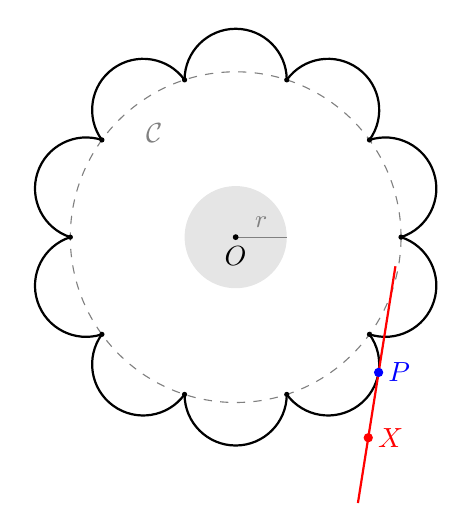
\begin{tikzpicture}[scale=1.05]
\pgfmathsetmacro{\rr}{2*sin(18)}\pgfmathsetmacro{\dd}{2*cos(18)}
\fill[gray!20] (0,0) circle (\rr);
\draw[gray,dashed] (0,0) circle (2);
\foreach \k in {0,...,9}{%
  \pgfmathsetmacro{\ph}{36*\k+18}%
  \draw[thick] (\ph:\dd) ++({\ph-90}:\rr) arc[start angle={\ph-90},end angle={\ph+90},radius=\rr];
  \fill ({36*\k}:2) circle (0.9pt);}
\draw[gray] (0,0) -- (\rr,0) node[midway,above]{\small $r$};
\fill (0,0) circle (1pt) node[below]{$O$};
\node[gray] at (128:1.6) {$\mathcal C$};
\pgfmathsetmacro{\ps}{-9}
\coordinate (M) at (-54:\dd);
\coordinate (P) at ([shift={(\ps:\rr)}]M);
\draw[red,thick] ([shift={({\ps+90}:1.3)}]P) -- ([shift={({\ps-90}:1.6)}]P);
\fill[blue] (P) circle (1.6pt) node[right,blue]{$P$};
\fill[red] ([shift={({\ps-90}:0.8)}]P) circle (1.6pt) node[right,red]{$X$};
\end{tikzpicture}\\[1mm]
{\small Zona gri: discul de rază $r=R\sin\frac{\pi}{n}$ în jurul lui $O$, prin care nu trece nicio tangentă.}
\end{center}}
\providecommand{\figpetaleint}{%
\begin{center}
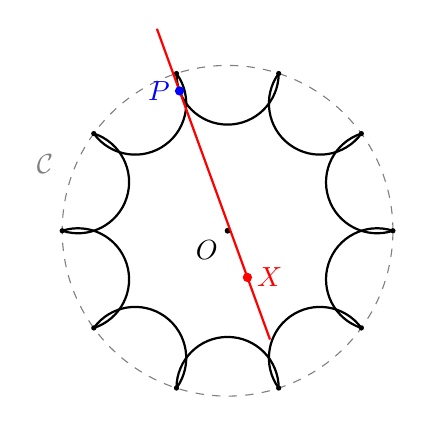
\begin{tikzpicture}[scale=1.05]
\pgfmathsetmacro{\rr}{2*sin(18)}\pgfmathsetmacro{\dd}{2*cos(18)}
\draw[gray,dashed] (0,0) circle (2);
\foreach \k in {0,...,9}{%
  \pgfmathsetmacro{\ph}{36*\k+18}%
  \draw[thick] (\ph:\dd) ++({\ph+90}:\rr) arc[start angle={\ph+90},end angle={\ph+270},radius=\rr];
  \fill ({36*\k}:2) circle (0.9pt);}
\fill (0,0) circle (1pt) node[below left]{$O$};
\node[gray] at (160:2.35) {$\mathcal C$};
\pgfmathsetmacro{\ps}{200}
\coordinate (M) at (90:\dd);
\coordinate (P) at ([shift={(\ps:\rr)}]M);
\draw[red,thick] ([shift={({\ps-90}:0.8)}]P) -- ([shift={({\ps+90}:3.2)}]P);
\fill[blue] (P) circle (1.6pt) node[left,blue]{$P$};
\fill[red] ([shift={({\ps+90}:2.4)}]P) circle (1.6pt) node[right,red]{$X$};
\end{tikzpicture}
\end{center}}

\prob{ojm}{OJM.17}{Planeta cu petale}
Fie $n\ge4$ și $A_1A_2\ldots A_n$ un poligon regulat înscris în cercul $\mathcal C$ de centru $O$ și rază $R$ (planeta). Pe fiecare latură $A_iA_{i+1}$ (cu $A_{n+1}=A_1$) construim, spre exteriorul lui $\mathcal C$, semicercul de diametru $A_iA_{i+1}$. Numim \emph{tangentă} orice dreaptă tangentă la unul dintre aceste semicercuri, inclusiv în capetele lui (în capete, tangenta este perpendiculara pe latură).
\begin{parti}
  \item Demonstrați că prin orice punct $X$ cu $OX\ge R$ trece o tangentă.
  \item Demonstrați că prin niciun punct $X$ cu $OX<R\sin\frac{\pi}{n}$ nu trece vreo tangentă. În particular, există puncte ale planetei prin care nu trece nicio tangentă.
\end{parti}
\figpetaleext
\vspace{1mm}\hrule

\prob{ojm}{OJM.18}{Planeta cu petale întoarse}
Fie $n\ge4$ și $A_1A_2\ldots A_n$ un poligon regulat înscris în cercul $\mathcal C$ de centru $O$ (planeta). Pe fiecare latură $A_iA_{i+1}$ (cu $A_{n+1}=A_1$) construim, spre \emph{interiorul} lui $\mathcal C$, semicercul de diametru $A_iA_{i+1}$. Un om se deplasează pe aceste semicercuri, în oricare sens, iar la un moment dat le părăsește și merge în linie dreaptă, pe tangenta la semicercul pe care se află. Demonstrați că omul poate ajunge în orice punct al planului, adică: prin orice punct $X$ al planului trece o dreaptă tangentă la unul dintre semicercuri (inclusiv în capetele lui).
\figpetaleint
\vspace{1mm}\hrule

\nivelE{onm}{Nivelul ONM}
\prob{onm}{ONM.1}{Clasică}
Arătați că numărul $\cos1$ este irațional.
\vspace{1mm}\hrule

\prob{onm}{ONM.2}{Inegalitatea lui Landau}
Fie $f:\mathbb{R}\to\mathbb{R}$ de două ori derivabilă, cu $|f(x)|\le M_0$ și $|f''(x)|\le M_2$ pentru orice $x\in\mathbb{R}$. Arătați că
\[ |f'(x)|\ \le\ 2\sqrt{M_0M_2}\qquad\text{pentru orice }x\in\mathbb{R}. \]
\vspace{1mm}\hrule

\prob{onm}{ONM.3}{}
Fie $f:\mathbb{R}\to\mathbb{R}$ o funcție derivabilă și \emph{strict convexă}, și fie $P\in\mathbb{R}[X]$ un polinom cu proprietatea
\[ f\bigl(P(x)\bigr)=f(x)\qquad\text{pentru orice }x\in\mathbb{R}. \]
\begin{parti}
  \item Arătați că, dacă $f'$ nu se anulează în niciun punct, atunci $P=X$.
  \item Determinați, în cazul general (adică fără ipoteza suplimentară de la (a)), toate polinoamele $P$ posibile.
\end{parti}
\vspace{1mm}\hrule

\prob{onm}{ONM.4}{}
Fie $(x_n)_{n\ge1}$ șirul de numere reale definit prin $x_1=1$ și
\[ 3x_{n+1}=\frac{x_n}{1!}+\frac{x_{n-1}}{2!}+\frac{x_{n-2}}{3!}+\cdots+\frac{x_1}{n!}\ ,\qquad n\ge1 . \]
Arătați că limita $\displaystyle\lim_{n\to\infty}\bigl(\ln4\bigr)^{n}x_n$ există și calculați-o.
\vspace{1mm}\hrule

\prob{onm}{ONM.5}{}
Fie $f:\mathbb{R}\to\mathbb{R}$ o funcție derivabilă cu proprietatea
\[ f(x)=1\quad\Longleftrightarrow\quad f'(x)=0\qquad\text{(pentru orice }x\in\mathbb{R}\text{)} . \]
Arătați că orice valoare $v\neq1$ este luată de $f$ în cel mult două puncte.
\vspace{1mm}\hrule

\prob{onm}{ONM.6}{Clasică}
Considerăm funcțiile derivabile $f:(0,\infty)\to\mathbb{R}$ cu proprietatea
\[ f'(x)=f\!\left(\frac1x\right)\qquad\text{pentru orice }x>0 . \]
\begin{parti}
  \item Arătați că o asemenea funcție este de două ori derivabilă și că $x^{2}f''(x)+f(x)=0$ pentru orice $x>0$.
  \item Determinați toate aceste funcții.
\end{parti}
\vspace{1mm}\hrule

\prob{onm}{ONM.7}{}
Determinați toate funcțiile derivabile $f:\mathbb{R}\to\mathbb{R}$ cu proprietatea
\[ f(x-y)=f(x)\,f'(y)-f'(x)\,f(y)\qquad\text{pentru orice }x,y\in\mathbb{R} . \]
\vspace{1mm}\hrule

\prob{onm}{ONM.8}{}
Determinați toate funcțiile $f:\mathbb{R}\to\mathbb{R}$ cu proprietatea lui Darboux pentru care
\[ f\bigl(f(x)\bigr)+f(x)=2x\qquad\text{pentru orice }x\in\mathbb{R} . \]
\vspace{1mm}\hrule

\prob{onm}{ONM.9}{}
Arătați că pentru orice $x>0$ are loc inegalitatea
\[ x^{1/x}+\left(\frac1x\right)^{x}\ \le\ 2 \]
și determinați cazul de egalitate.
\vspace{1mm}\hrule

\prob{onm}{ONM.10}{}
Fie $x_1=1$ și
\[ x_{n+1}=x_n+\frac{1}{x_1+x_2+\cdots+x_n}\ ,\qquad n\ge1 . \]
\begin{parti}
  \item Arătați că $x_n\to\infty$ și că $\displaystyle\lim_{n\to\infty}\frac{x_n^{2}}{\ln n}=2$.
  \item Arătați că șirul $\bigl(x_n^{2}-2\ln n-\ln\ln n\bigr)_{n\ge2}$ este convergent.
\end{parti}
\vspace{1mm}\hrule

\prob{onm}{ONM.11}{}
Fie $x_1>0$ și
\[ x_{n+1}=x_n+\frac{2n}{x_n}\ ,\qquad n\ge1 . \]
\begin{parti}
  \item Arătați că $\displaystyle\lim_{n\to\infty}\bigl(x_n-n\sqrt2\bigr)=0$.
  \item Arătați că șirul $\bigl(n\,(x_n-n\sqrt2)\bigr)_{n\ge1}$ este convergent și că limita sa este nulă dacă și numai dacă $x_1=\sqrt2$.
\end{parti}
\vspace{1mm}\hrule

\subsectiuneclasa{Puntea între a XI-a și a XII-a}{Șiruri rezolvate cu integrale: sume Riemann, comparare cu integrala, asimptotică, ecuații diferențiale elementare.}{Enunțuri · Puntea XI--XII}
\nivelE{olm}{Nivelul OLM}
\prob{olm}{OLM.1}{Clasică}
Fie $S_n=\dfrac1{n+1}+\dfrac1{n+2}+\cdots+\dfrac1{2n}$, $n\ge1$.
\begin{parti}
  \item Calculați $\displaystyle\lim_{n\to\infty}S_n$.
  \item Calculați $\displaystyle\lim_{n\to\infty}n\bigl(\ln2-S_n\bigr)$.
\end{parti}
\vspace{1mm}\hrule

\prob{olm}{OLM.2}{}
Fie $f:[0,1]\to\mathbb{R}$ o funcție de două ori derivabilă, cu
\[ f''(x)=f(x)\,f'(x)\quad\text{pentru orice }x\in[0,1],\qquad f(0)=f(1)=0 . \]
Arătați că $f'(1)=f'(0)$.
\vspace{1mm}\hrule

\prob{olm}{OLM.3}{}
Calculați $\left\lfloor\displaystyle\sum_{k=1}^{10^6}\frac1{\sqrt k}\right\rfloor$.
\vspace{1mm}\hrule

\prob{olm}{OLM.4}{}
Notăm $H_{n}=1+\dfrac12+\dfrac13+\cdots+\dfrac1n$. Arătați că șirul
\[ x_{n}=H_{n^{2}}-2H_{n} \]
este convergent și calculați limita sa.
\vspace{1mm}\hrule

\prob{olm}{OLM.5}{}
Calculați $\displaystyle\lim_{n\to\infty}\ n\sum_{k=n+1}^{\infty}\frac1{k^2}$.
\vspace{1mm}\hrule

\prob{olm}{OLM.6}{}
Calculați
\[ \lim_{x\to0}\frac{e^{x^2/2}\cos x-1}{x^4} . \]
\vspace{1mm}\hrule

\prob{olm}{OLM.7}{}
Arătați că șirul $s_n=\displaystyle\sum_{k=1}^{n}\sin\frac1k-\ln n$ este convergent.
\vspace{1mm}\hrule

\nivelE{ojm}{Nivelul OJM}
\prob{ojm}{OJM.1}{}
Determinați numerele reale $x>0$ pentru care seria
\[ \sum_{n\ge1}\frac{n!\ x^{\,n}}{n^{\,n}} \]
este convergentă.
\vspace{1mm}\hrule

\prob{ojm}{OJM.2}{}
Fie $f:[0,1]\to\mathbb{R}$ o funcție de două ori derivabilă, cu derivata a doua continuă, care satisface
\[ f''(x)=e^{\,x}f(x)\quad\text{pentru orice }x\in[0,1],\qquad f(0)=f(1)=0 . \]
Arătați că $f$ este identic nulă.
\vspace{1mm}\hrule

\prob{ojm}{OJM.3}{}
Determinați toate funcțiile derivabile $f:\mathbb{R}\to\mathbb{R}$ cu $f(0)=1$ și
\[ f'(x)\cdot f(-x)=1\qquad\text{pentru orice }x\in\mathbb{R} . \]
\vspace{1mm}\hrule

\prob{ojm}{OJM.4}{}
Fie $x_{1}\in(0,1)$ și
\[ x_{n+1}=x_{n}-x_{n}^{3}\ ,\qquad n\ge1 . \]
\begin{parti}
  \item Calculați $\displaystyle\lim_{n\to\infty}\bigl(x_{1}^{3}+x_{2}^{3}+\cdots+x_{n}^{3}\bigr)$.
  \item Calculați $\displaystyle\lim_{n\to\infty}n\,x_{n}^{2}$.
  \item Calculați $\displaystyle\lim_{n\to\infty}\frac{x_{1}^{2}+x_{2}^{2}+\cdots+x_{n}^{2}}{\ln n}$.
\end{parti}
\vspace{1mm}\hrule

\prob{ojm}{OJM.5}{}
Determinați toate funcțiile continue $f:(-1,1)\to\mathbb{R}$ cu proprietatea
\[ f\bigl(x^{2}\bigr)=f(x)+x\qquad\text{pentru orice }x\in(-1,1) . \]
\vspace{1mm}\hrule

\prob{ojm}{OJM.6}{}
Fie $x_1\in\mathbb{R}$ și
\[ x_{n+1}=\frac{x_n^{2}+x_n}{x_n^{2}+1}\ ,\qquad n\ge1 . \]
\begin{parti}
  \item Arătați că, dacă $x_1>0$, atunci șirul este convergent și calculați limita sa.
  \item Arătați că, dacă $x_1\in(-1,0)$, atunci șirul este convergent și calculați $\displaystyle\lim_{n\to\infty}n\,x_n$.
\end{parti}
\vspace{1mm}\hrule

\prob{ojm}{OJM.7}{Clasică}
Fie $x_1=1$ și $x_{n+1}=x_n+\dfrac{1}{x_n}$ pentru $n\ge1$.
\begin{parti}
  \item Arătați că $\displaystyle\lim_{n\to\infty}\frac{x_n}{\sqrt{2n}}=1$.
  \item Arătați că $\displaystyle\lim_{n\to\infty}\frac{x_n^{2}-2n}{\ln n}=\frac12$.
\end{parti}
\vspace{1mm}\hrule

\prob{ojm}{OJM.8}{}
Fie $\alpha>0$ un număr real fixat și $S_{n}=1^{\alpha}+2^{\alpha}+\cdots+n^{\alpha}$. Arătați că
\[ \lim_{n\to\infty}\ n\left(\frac{S_{n}}{n^{\alpha+1}}-\frac{1}{\alpha+1}\right)=\frac12 . \]
\vspace{1mm}\hrule

\prob{ojm}{OJM.9}{}
Arătați că \emph{nu există} nicio funcție $f:[0,1]\to\mathbb{R}$, de două ori derivabilă și cu derivata a doua continuă, care să satisfacă simultan
\[ f''(x)+\pi^{2}f(x)=\sin(\pi x)\quad\text{pentru orice }x\in[0,1],\qquad f(0)=f(1)=0 . \]
\vspace{1mm}\hrule

\nivelE{onm}{Nivelul ONM}
\prob{onm}{ONM.1}{Clasică}
Pentru $n\ge1$, fie
\[ x_n=\frac{1}{e^{\,n}}\sum_{i=0}^{n}\frac{n^{\,i}}{i!} \]
(adică raportul dintre suma \emph{primilor $n+1$ termeni} din dezvoltarea în serie Taylor a lui $e^{\,n}$ și $e^{\,n}$ însuși). Arătați că șirul $(x_n)$ este convergent și calculați limita sa.
\vspace{1mm}\hrule

\prob{onm}{ONM.2}{}
Fie $u_{1}>0$ și
\[ u_{n+1}=\sqrt[n]{\,u_{n}^{\,n}+n^{\,n}\,}\ ,\qquad n\ge1 . \]
Arătați că șirul $\bigl(u_{n}-n\bigr)_{n\ge1}$ este convergent și calculați limita sa.
\vspace{1mm}\hrule

\prob{onm}{ONM.3}{}
Pentru $N\ge1$ și $0\le a<b<2\pi$, notăm cu $S_N(a,b)$ numărul indicilor $n\le N$ pentru care $\sqrt n$, redus modulo $2\pi$, cade în intervalul $[a,b)$.
\begin{parti}
  \item Arătați că
  \[ S_N(a,b)=\frac{b-a}{2\pi}\,N+O\bigl(\sqrt N\bigr) , \]
  unde notația $O\bigl(\sqrt N\bigr)$ desemnează o cantitate al cărei modul este cel mult $C\sqrt N$, pentru o constantă $C$ ce nu depinde de $N$ (poate depinde de $a$ și $b$).
  \item Arătați că, pentru orice $-1\le u<v\le1$,
  \[ \lim_{N\to\infty}\frac{1}{N}\cdot\#\Bigl\{\,n\le N\ :\ \sin\sqrt n\in[u,v)\,\Bigr\}=\frac{\arcsin v-\arcsin u}{\pi} , \]
  și că, în particular, orice $c\in[-1,1]$ este punct limită al șirului $\bigl(\sin\sqrt n\bigr)_{n\ge1}$.
\end{parti}
\vspace{1mm}\hrule
